%%
%% Beginning of file 'sample62.tex'
%%
%% Modified 2018 January
%%
%% This is a sample manuscript marked up using the
%% AASTeX v6.2 LaTeX 2e macros.
%%
%% AASTeX is now based on Alexey Vikhlinin's emulateapj.cls 
%% (Copyright 2000-2015). See the classfile for details.

%% AASTeX requires revtex4-1.cls (http://publish.aps.org/revtex4/) and
%% other external packages (latexsym, graphicx, amssymb, longtable, and epsf).
%% All of these external packages should already be present in the modern TeX 
%% distributions. If not they can also be obtained at www.ctan.org.

%% The first piece of markup in an AASTeX v6.x document is the \documentclass
%% command. LaTeX will ignore any data that comes before this command. The 
%% documentclass can take an optional argument to modify the output style.
%% The command below calls the preprint style which will produce a tightly 
%% typeset, one-column, single-spaced document. It is the default and thus
%% does not need to be explicitly stated.
%%
%%
%% using aastex version 6.2
\documentclass[column]{aastex62}

\usepackage{xcolor}
\usepackage{amsmath}
\usepackage{graphicx}
\usepackage[normalem]{ulem}

%% The default is a single spaced, 10 point font, single spaced article.
%% There are 5 other style options available via an optional argument. They
%% can be envoked like this:
%%
%% \documentclass[argument]{aastex62}
%% 
%% where the layout options are:
%%
%% twocolumn  : two text columns, 10 point font, single spaced article.
%%                This is the most compact and represent the final published
%%                derived PDF copy of the accepted manuscript from the publisher
%%  manuscript  : one text column, 12 point font, double spaced article.
%%  preprint    : one text column, 12 point font, single spaced article.
%%  preprint2   : two text columns, 12 point font, single spaced article.
%%  modern      : a stylish, single text column, 12 point font, article with
%%                wider left and right margins. This uses the Daniel
%%                Foreman-Mackey and David Hogg design.
%%  RNAAS       : Preferred style for Research Notes which are by design 
%%                lacking an abstract and brief. DO NOT use \begin{abstract}
%%                and \end{abstract} with this style.
%%
%% Note that you can submit to the AAS Journals in any of these 6 styles.
%%
%% There are other optional arguments one can envoke to allow other stylistic
%% actions. The available options are:
%%
%%  astrosymb    : Loads Astrosymb font and define \astrocommands. 
%%  tighten      : Makes baselineskip slightly smaller, only works with 
%%                 the twocolumn substyle.
%%  times        : uses times font instead of the default
%%  linenumbers  : turn on lineno package.
%%  trackchanges : required to see the revision mark up and print its output
%%  longauthor   : Do not use the more compressed footnote style (default) for 
%%                 the author/collaboration/affiliations. Instead print all
%%                 affiliation information after each name. Creates a much
%%                 long author list but may be desirable for short author papers
%%
%% these can be used in any combination, e.g.
%%
%% \documentclass[twocolumn,linenumbers,trackchanges]{aastex62}
%%
%% AASTeX v6.* now includes \hyperref support. While we have built in specific
%% defaults into the classfile you can manually override them with the
%% \hypersetup command. For example,
%%
%%\hypersetup{linkcolor=red,citecolor=green,filecolor=cyan,urlcolor=magenta}
%%
%% will change the color of the internal links to red, the links to the
%% bibliography to green, the file links to cyan, and the external links to
%% magenta. Additional information on \hyperref options can be found here:
%% https://www.tug.org/applications/hyperref/manual.html#x1-40003
%%
%% If you want to create your own macros, you can do so
%% using \newcommand. Your macros should appear before
%% the \begin{document} command.
%%
\newcommand{\vdag}{(v)^\dagger}
\newcommand\aastex{AAS\TeX}
\newcommand\latex{La\TeX}
\newcommand\todo[1]{\textcolor{red}{#1}}
\newcommand\nt[1]{\textcolor{red}{#1}}
\newcommand\st[1]{\sout{#1}}
\newcommand{\cc}{\textcolor{red}{\scriptsize{(citation needed)}}}
\newcommand{\tnp}[1]{\textcolor{brown}{\scriptsize{( #1~ \textbf{ -- TNP})}}}

%% Reintroduced the \received and \accepted commands from AASTeX v5.2
\received{\today}
%\revised{January 7, 2018}
%\accepted{\today}
%% Command to document which AAS Journal the manuscript was submitted to.
%% Adds "Submitted to " the arguement.
%%\submitjournal{ApJ}

%% Mark up commands to limit the number of authors on the front page.
%% Note that in AASTeX v6.2 a \collaboration call (see below) counts as
%% an author in this case.
%
%\AuthorCollaborationLimit=3
%
%% Will only show Schwarz, Muench and "the AAS Journals Data Scientist 
%% collaboration" on the front page of this example manuscript.
%%
%% Note that all of the author will be shown in the published article.
%% This feature is meant to be used prior to acceptance to make the
%% front end of a long author article more manageable. Please do not use
%% this functionality for manuscripts with less than 20 authors. Conversely,
%% please do use this when the number of authors exceeds 40.
%%
%% Use \allauthors at the manuscript end to show the full author list.
%% This command should only be used with \AuthorCollaborationLimit is used.

%% The following command can be used to set the latex table counters. It
%% is needed in this document because it uses a mix of latex tabular and
%% AASTeX deluxetables. In general it should not be needed.
%\setcounter{table}{1}

%%%%%%%%%%%%%%%%%%%%%%%%%%%%%%%%%%%%%%%%%%%%%%%%%%%%%%%%%%%%%%%%%%%%%%%%%%%%%%%%
%%
%% The following section outlines numerous optional output that
%% can be displayed in the front matter or as running meta-data.
%%
%% If you wish, you may supply running head information, although
%% this information may be modified by the editorial offices.
%\shorttitle{}
%%\shortauthors{}
%%
%% You can add a light gray and diagonal water-mark to the first page 
%% with this command:
% \watermark{text}
%% where "text", e.g. DRAFT, is the text to appear. If the text is 
%% long you can control the water-mark size with:
% \setwatermarkfontsize{dimension}
%% where dimension is any recognized LaTeX dimension, e.g. pt, in, etc.
%%
%%%%%%%%%%%%%%%%%%%%%%%%%%%%%%%%%%%%%%%%%%%%%%%%%%%%%%%%%%%%%%%%%%%%%%%%%%%%%%%%

%% This is the end of the preamble. Indicate the beginning of the
%% manuscript itself with \begin{document}.
\begin{document}

	\title{KAW instability and some other stuff}
	%% LaTeX will automatically break titles if they run longer than
	%% one line. However, you may use \\ to force a line break if
	%% you desire. In v6.2 you can include a footnote in the title.
	
	%% A significant change from earlier AASTEX versions is in the structure for 
	%% calling author and affilations. The change was necessary to implement 
	%% autoindexing of affilations which prior was a manual process that could 
	%% easily be tedious in large author manuscripts.
	%%
	%% The \author command is the same as before except it now takes an optional
	%% arguement which is the 16 digit ORCID. The syntax is:
	%% \author[xxxx-xxxx-xxxx-xxxx]{Author Name}
	%%
	%% This will hyperlink the author name to the author's ORCID page. Note that
	%% during compilation, LaTeX will do some limited checking of the format of
	%% the ID to make sure it is valid.
	%%
	%% Use \affiliation for affiliation information. The old \affil is now 
	%% aliased to \affiliation. AASTeX v6.2 will automatically index these in 
	%% the header. When a duplicate is found its index will be the same as its 
	%% previous entry.
	%%
	%% Note that \altaffilmark and \altaffiltext have been removed and thus 
	%% can not be used to document secondary affiliations. If they are used latex
	%% will issue a specific error message and quit. Please use multiple 
	%% \affiliation calls for to document more than one affiliation.
	%%
	%% The new \altaffiliation can be used to indicate some secondary information
	%% such as fellowships. This command produces a non-numeric footnote that is
	%% set away from the numeric \affiliation footnotes. NOTE that if an
	%% \altaffiliation command is used it must come BEFORE the \affiliation call,
	%% right after the \author command, in order to place the footnotes in
	%% the proper location.
	%%
	%% Use \email to set provide email addresses. Each \email will appear on its
	%% own line so you can put multiple email address in one \email call. A new
	%% \correspondingauthor command is available in V6.2 to identify the
	%% corresponding author of the manuscript. It is the author's responsibility
	%% to make sure this name is also in the author list.
	%%
	%% While authors can be grouped inside the same \author and \affiliation
	%% commands it is better to have a single author for each. This allows for
	%% one to exploit all the new benefits and should make book-keeping easier.
	%%
	%% If done correctly the peer review system will be able to
	%% automatically put the author and affiliation information from the 
	%% manuscript and save the corresponding author the trouble of entering it
	%% by hand.
	
	\author{UD-Plasma Group}
	\affiliation{Department of Physics and Astronomy, University of Delaware, Newark, DE 19716, USA}
    %\email{ahmadr@udel.edu}

	%% Note that the \and command from previous versions of AASTeX is now
	%% depreciated in this version as it is no longer necessary. AASTeX 
	%% automatically takes care of all commas and "and"s between authors names.
		
	%% AASTeX 6.2 has the new \collaboration and \nocollaboration commands to
	%% provide the collaboration status of a group of authors. These commands 
	%% can be used either before or after the list of corresponding authors. The
	%% argument for \collaboration is the collaboration identifier. Authors are
	%% encouraged to surround collaboration identifiers with ()s. The 
	%% \nocollaboration command takes no argument and exists to indicate that
	%% the nearby authors are not part of surrounding collaborations.
		
	%% Mark off the abstract in the ``abstract'' environment.
	\begin{abstract}
		I am adding some figures!

		\keywords{plasmas --- turbulence --microinstabilities}

	\end{abstract}

	%% From the front matter, we move on to the body of the paper.
	%% Sections are demarcated by \section and \subsection, respectively.
	%% Observe the use of the LaTeX \label
	%% command after the \subsection to give a symbolic KEY to the
	%% subsection for cross-referencing in a \ref command.
	%% You can use LaTeX's \ref and \label commands to keep track of
	%% cross-references to sections, equations, tables, and figures.
	%% That way, if you change the order of any elements, LaTeX will
	%% automatically renumber them.
	%%
	%% We recommend that authors also use the natbib \citep
	%% and \citet commands to identify citations. The citations are
	%% tied to the reference list via symbolic KEYs. The KEY corresponds
	%% to the KEY in the \bibitem in the reference list below. 

	\section{Introduction} \label{sec:intro}
	
        Added a few figures and updated a few others!		

		\begin{figure*}
			\begin{center}
				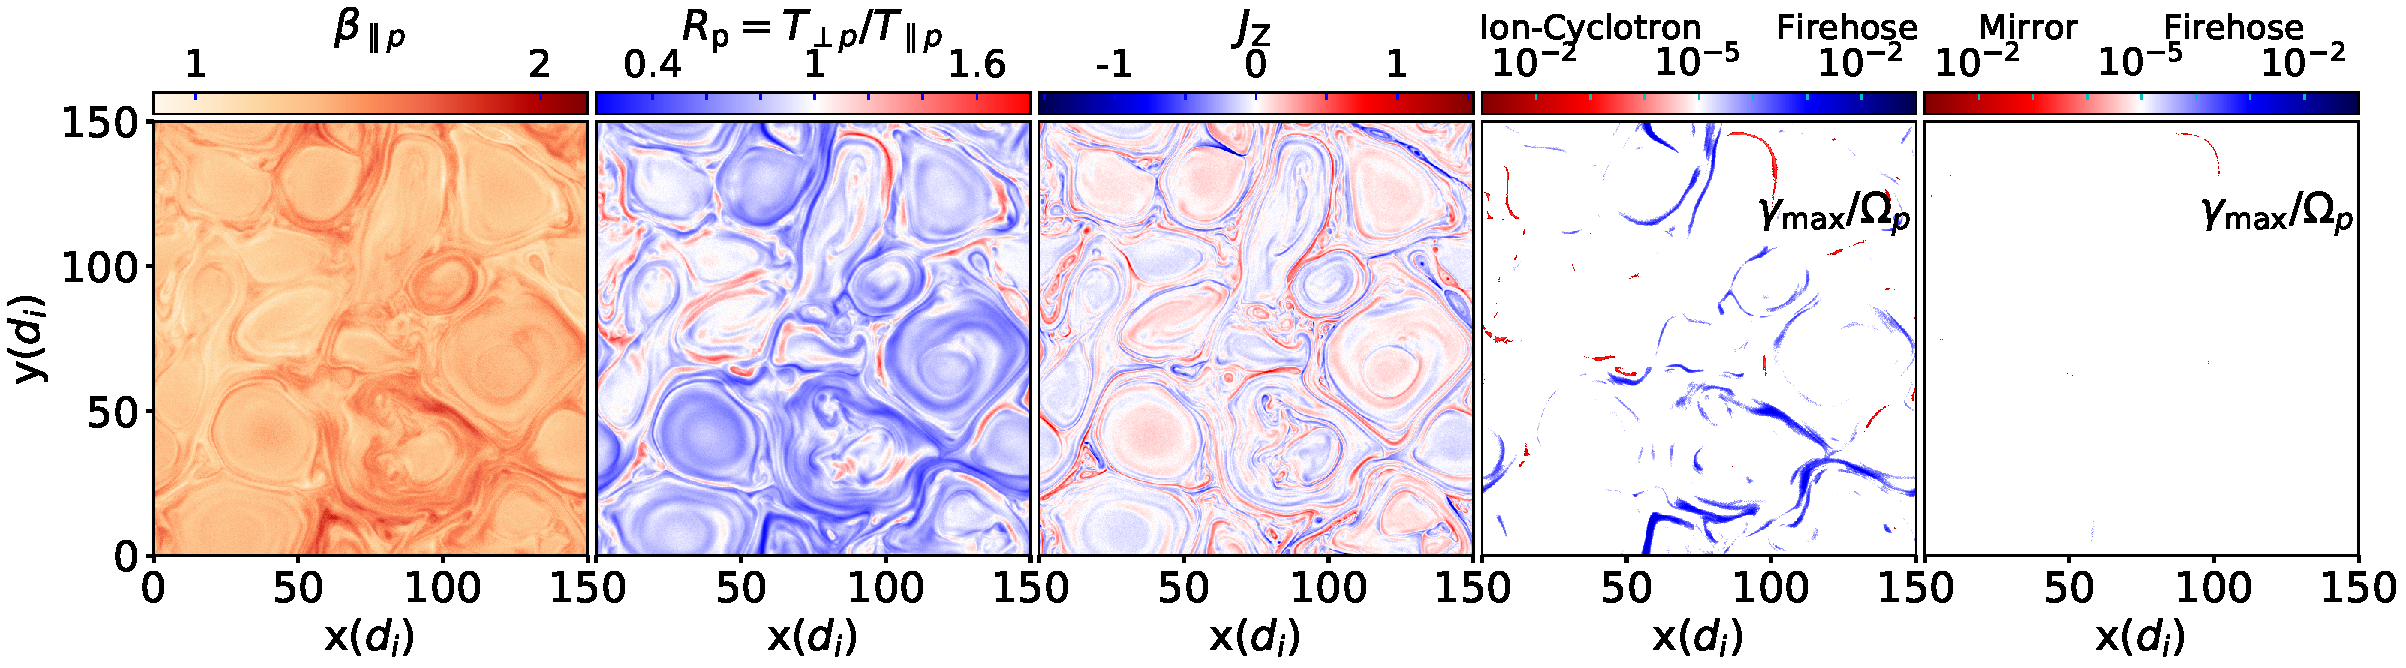
\includegraphics[width=1.05\textwidth,
				angle=0]{b_r_j_gamma_all_gamma_k_149p6_hb.pdf}
				\caption{Plot of various parameters for the 2-D PIC simulation for in plane fluctuations in magnetic field}
				\label{fig:brj1}
			\end{center}
		\end{figure*}

        \begin{figure*}
			\begin{center}
				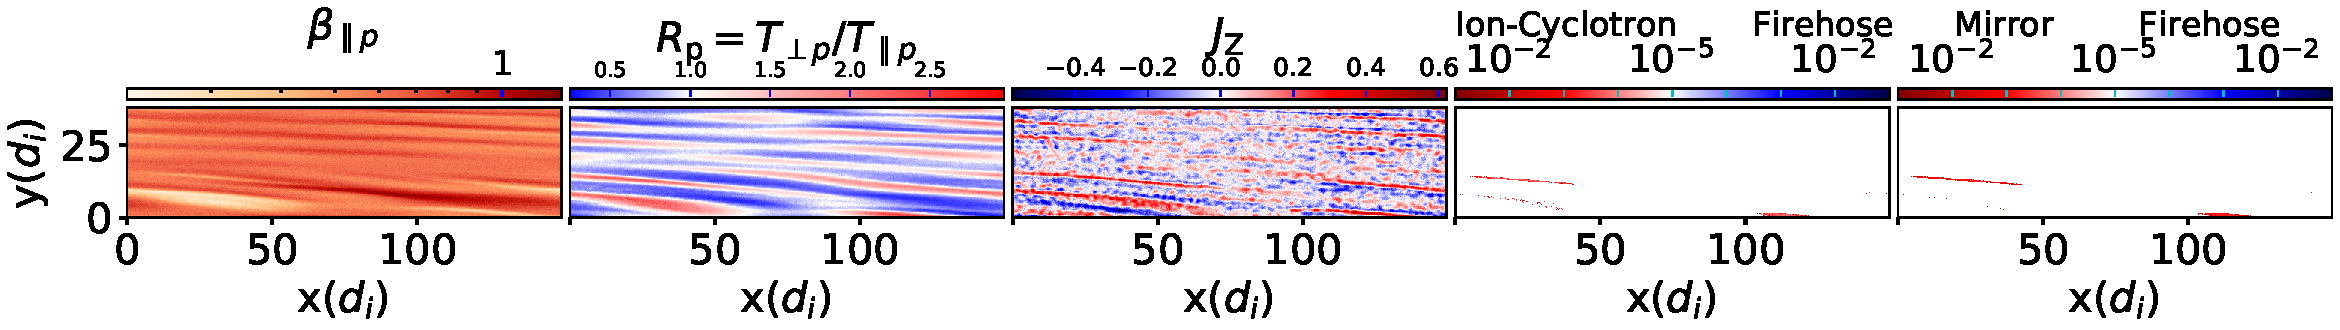
\includegraphics[width=1.05\textwidth, height=3.1cm,
				angle=0]{b_r_j_gamma_all_kaw_ti0p6te0p6_Time6000wpe_2.pdf}
				\caption{Plot of various parameters for the 2-D PIC simulation for out of the plane fluctuations in magnetic field}
				\label{fig:brj2}
			\end{center}
		\end{figure*}

    Comparing the two 2-D simulations (in-plane Figure \ref{fig:brj1} and out of plane Figure \ref{fig:brj2} fluctuations) we see that despite having smaller $\beta_{\parallel p}$ for out of plane fluctuations, we get a lot more mirror modes than what we got for in-plane fluctuation. I haven't quantified it yet, but this should be easy to do. Taking the ratio of number of ion-cyclotron modes to mirror modes might present a fair comparison between the two.
    
    I have added the brazil-plots for all three cases here, 2-D PIC in (\ref{fig:brz2dip}) and out of plane (\ref{fig:brz2dpp}) fluctuation as well as 3-D Pic (\ref{fig:brz3d}), with threshold over plotted on them. For actual spacecraft data, brazil-plots could be found in \citet{Maruca2018} (for magnetosheath) and \citet{Hellinger2006} (for solar wind).

		\begin{figure*}
			\begin{center}
				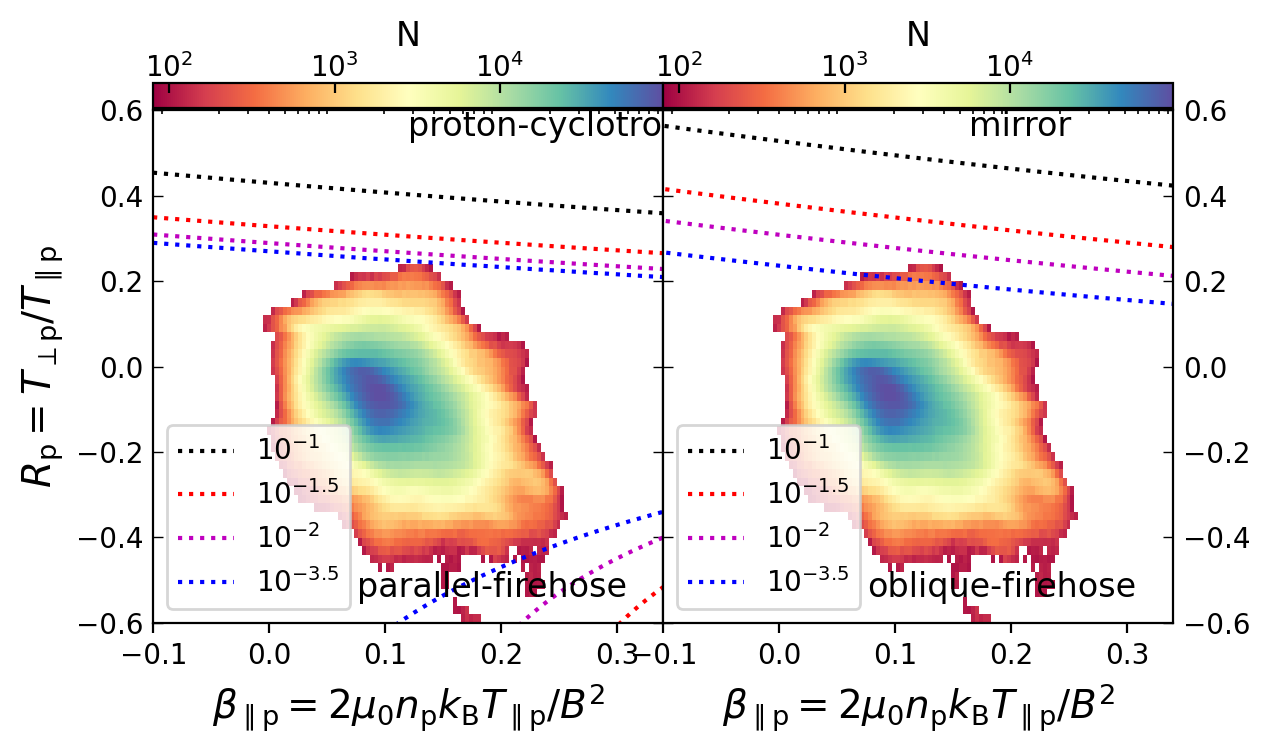
\includegraphics[width=0.9\textwidth]{brzl_thresh_149p6_hb.png}
				\caption{Brazil plot for 2D simulation (in plane magnetic fluctuations). Legend of lines are the associated growth rates.}
				\label{fig:brz2dip}
			\end{center}
		\end{figure*}

		\begin{figure*}
			\begin{center}
				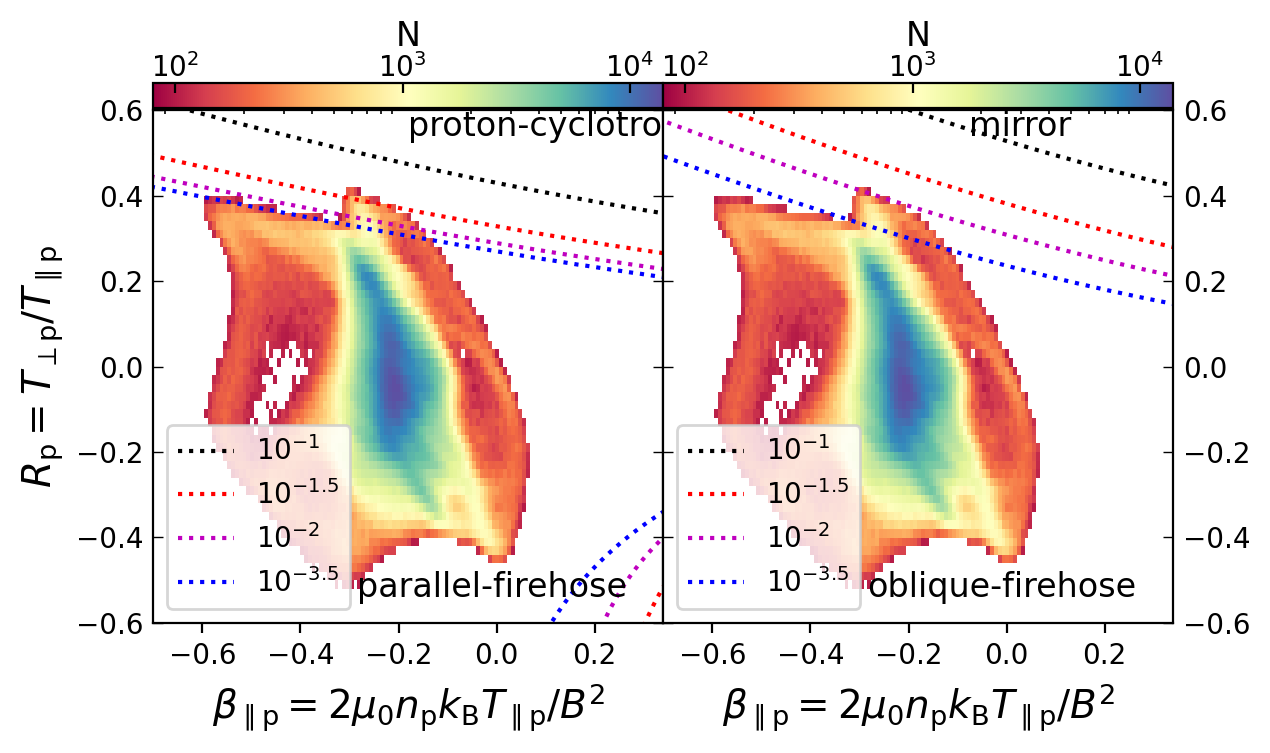
\includegraphics[width=0.9\textwidth]{brzl_thresh_ti0p6te0p6_Time6000wpe.png}
				\caption{Brazil plot for 2D simulation (out of plane magnetic fluctuations). Legend of lines are the associated growth rates.}
				\label{fig:brz2dpp}
			\end{center}
		\end{figure*}

		\begin{figure*}
			\begin{center}
				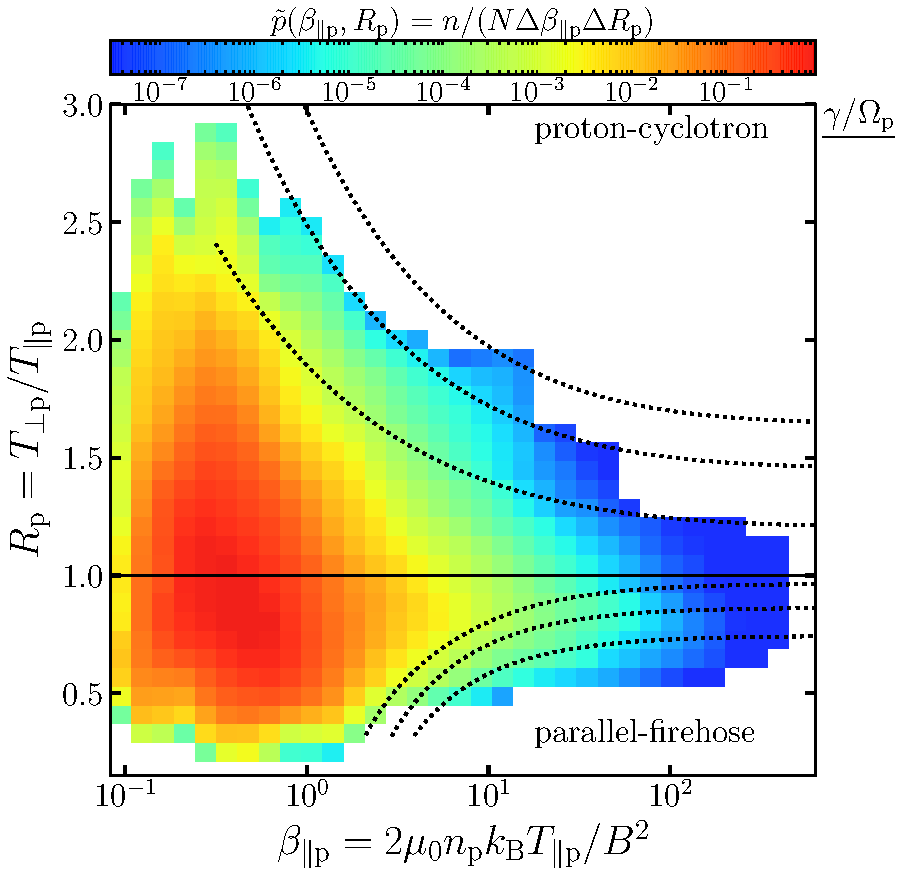
\includegraphics[width=0.49\textwidth]{brazil_prob_pic_parallel.pdf}
				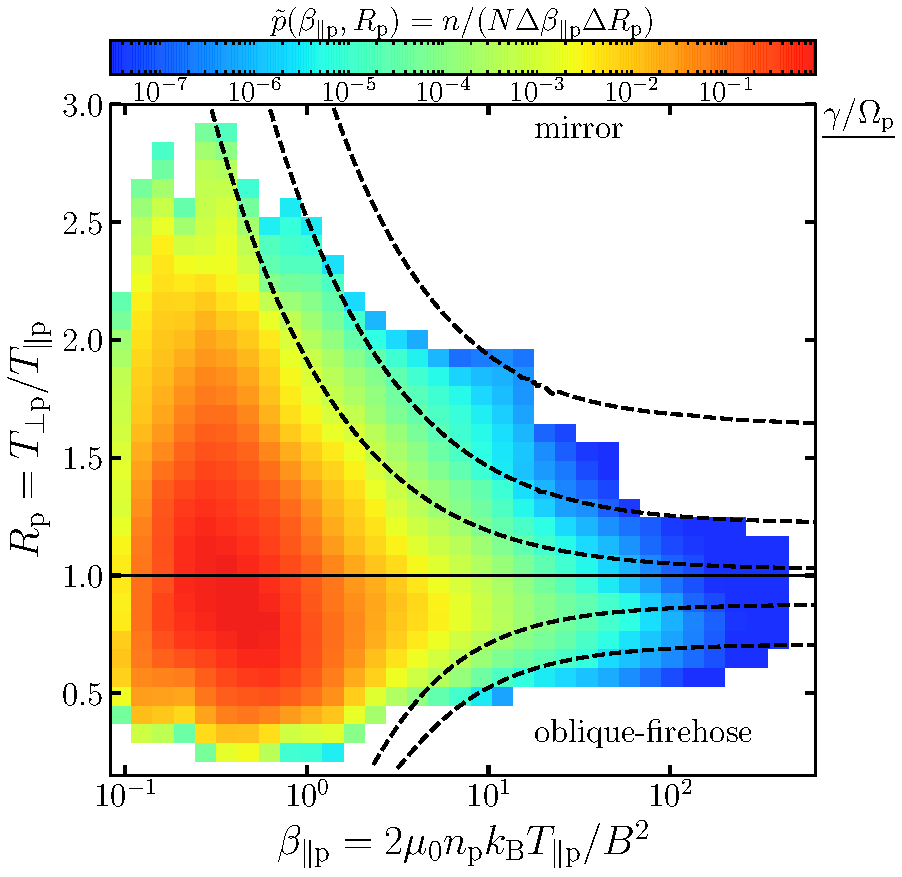
\includegraphics[width=0.49\textwidth]{brazil_prob_pic_oblique.pdf}
				\caption{Brazil plot for 3D simulation.}
				\label{fig:brz3d}
			\end{center}
		\end{figure*}

    \clearpage
	\section{PDFs and PVIs} \label{sec:pdf}
	
	    \subsection{PDF} \label{sec:pdf}
    	    As Bill suggested I made PDFs of some of the parameters for the three different cases. I have yet to do it for MMS observations and possibly WIND, partly because that will need some tweaking in the code since MMS data (and WIND data), unlike simulation ones, are time-series. Figure \ref{fig:pdfs} shows this for three different cases. $2D-\parallel$ is the case where fluctuations in magnetic field are parallel to $\Vec{B}_0$ whereas $2D-\pperp$ is the case where fluctuations in magnetic field are perpendicular to $\Vec{B}_0$. The black line is the best fit to PDF from 3-D simulation and its legend is the slope of the best fit line in log-log scale. For the non-propagating instabilities, it can be observed that as $\gamma$ gets larger than 0.1, we see a spike in PDF implying presence of a lot of excited modes. Either this actually happens or is some quirk of the code. Hopefully Ben or Peter will be able to shed some more light on this. PDFs of $R_p$ for three cases are similar in shape and is very Gaussian like. However for $\beta_{\parallel p}$ the shapes vary widely.\\

		\begin{figure*}
			\begin{center}
				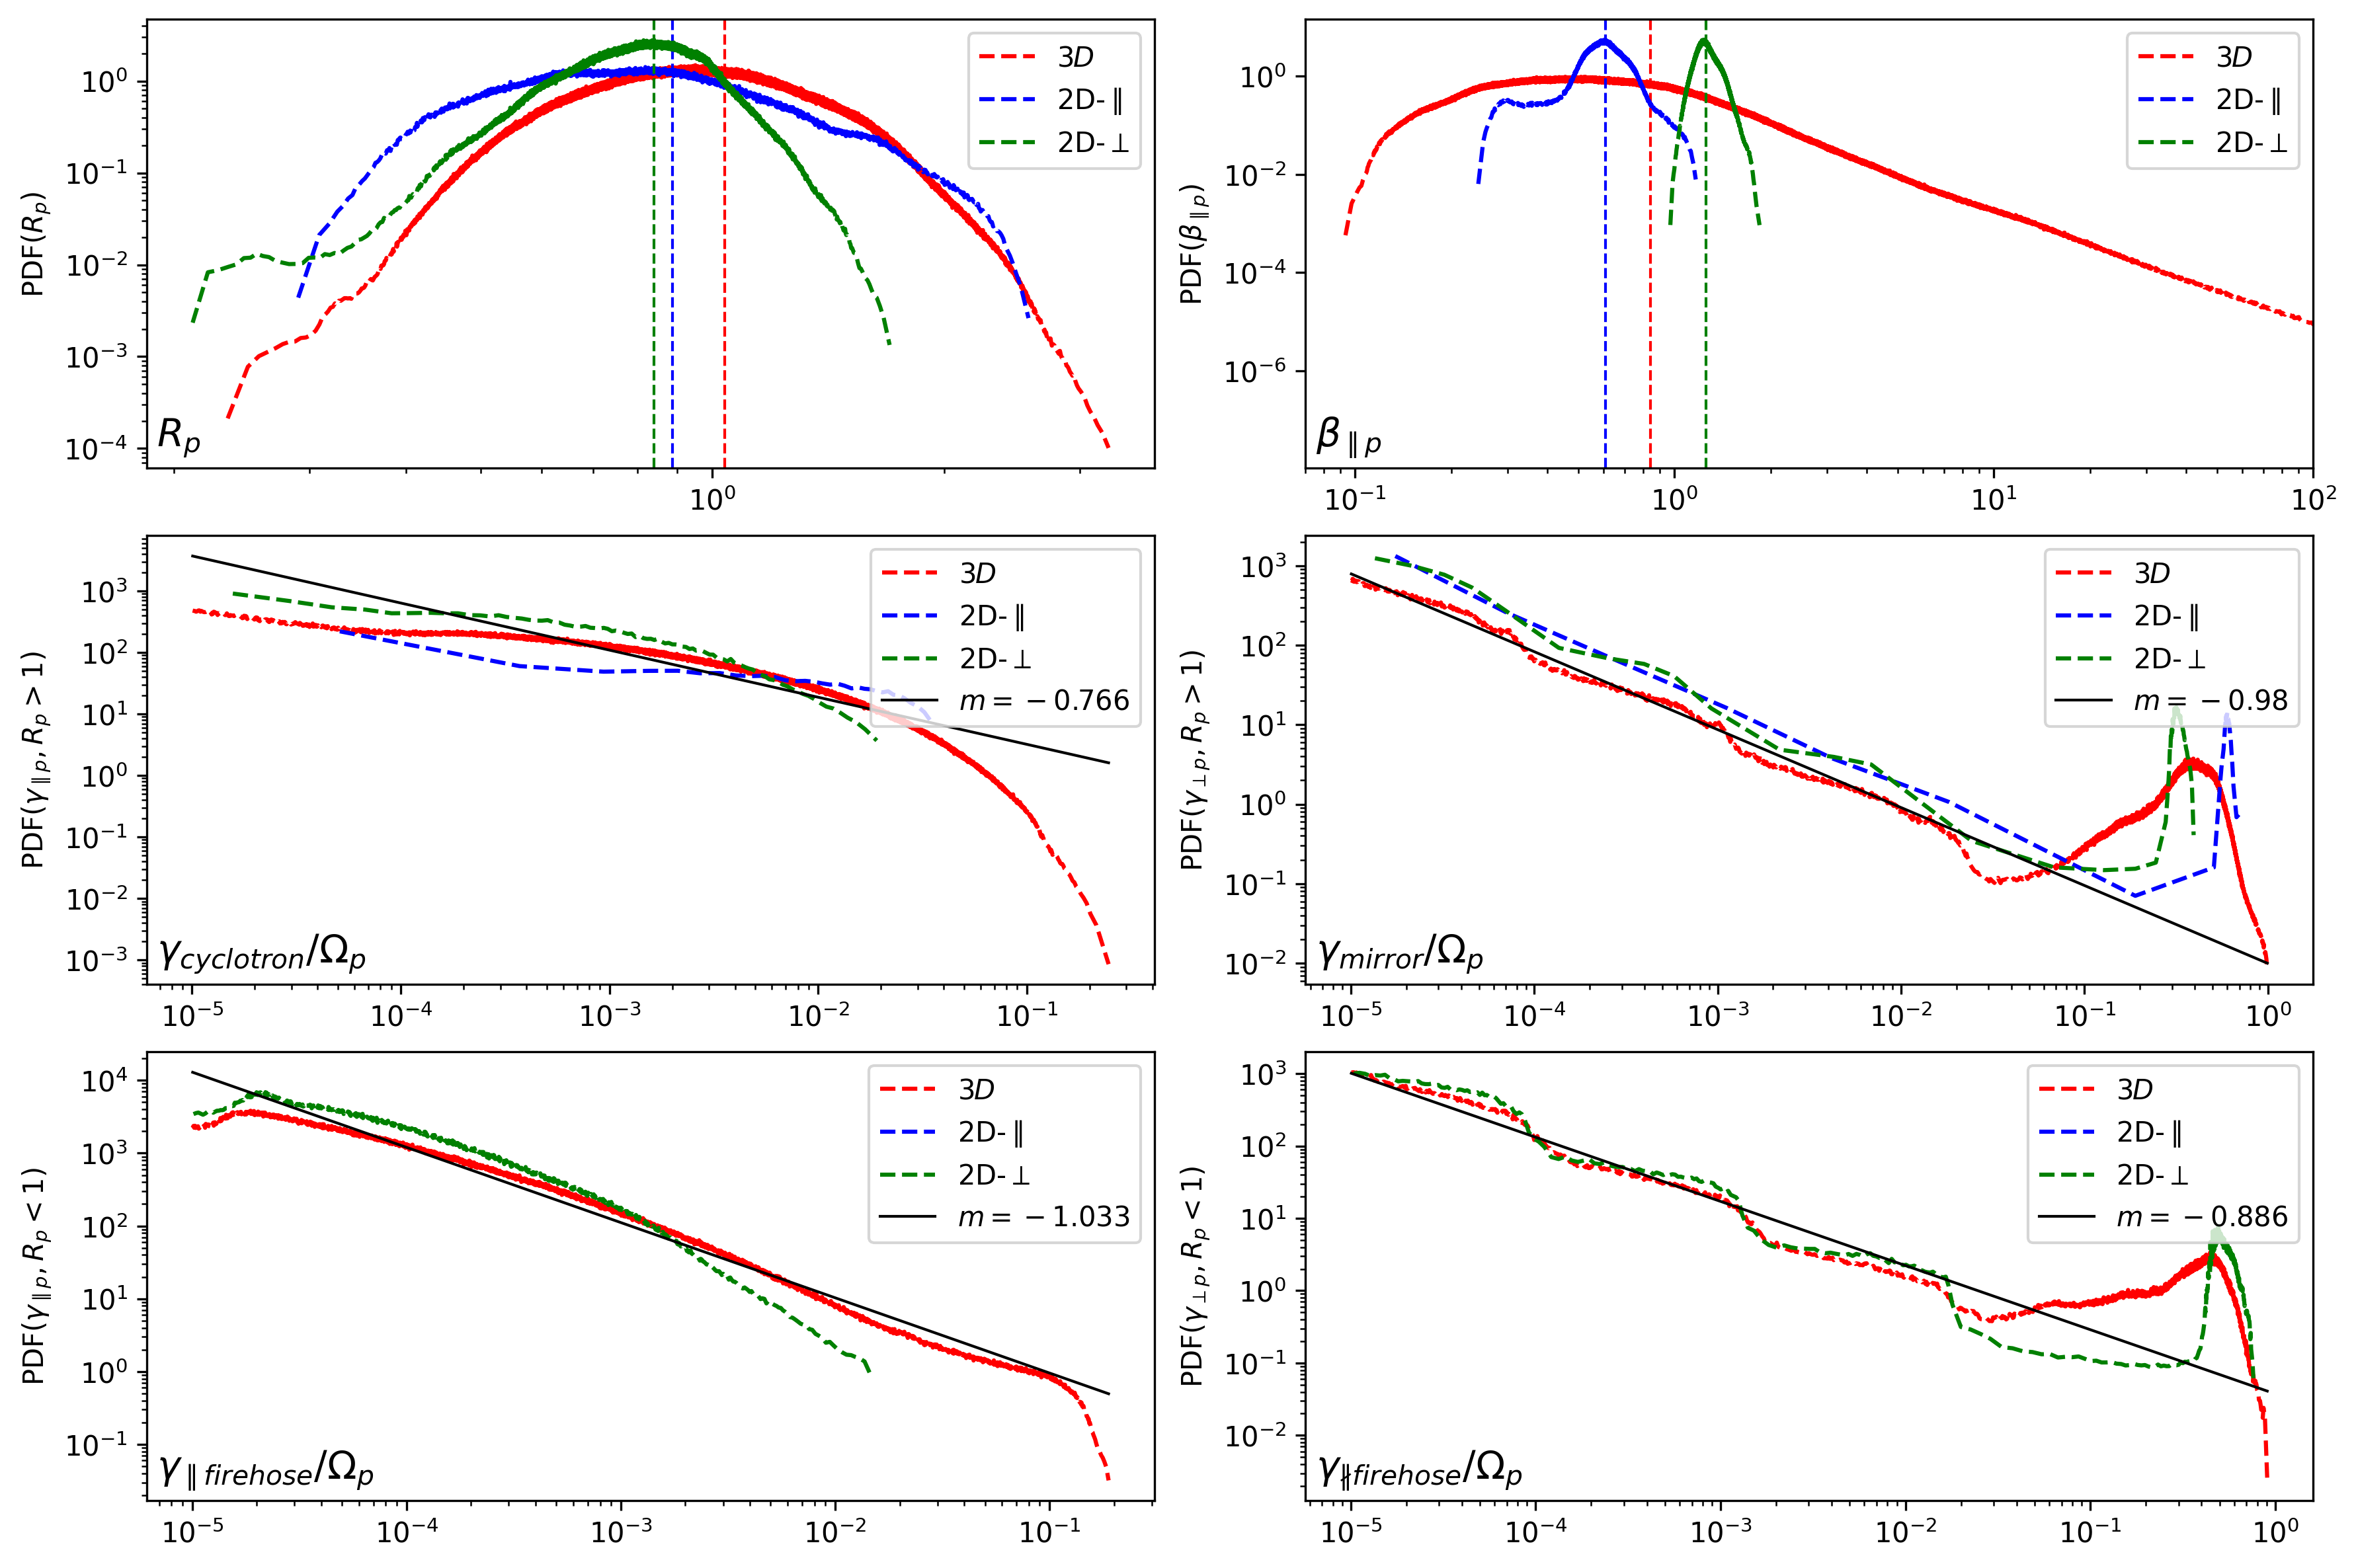
\includegraphics[width=1.05\textwidth]{pdfs.png}
				\caption{PDFs of various parameters like $R_p, \beta_{\parallel p}, \mathrm{and} \gamma$ The black line is the best fit to PDF from 3-D simulation and its legend is the slope of the best fit line in log-log scale. Please note that for fitting I only considered values such that $\gamma/\Omega_p <0.1$}
				\label{fig:pdfs}
			\end{center}
		\end{figure*}

        \subsection{PVI} \label{sec:pvi}
            I also made plots of the PVI for the two 2D-simulations (Figures \ref{fig:pvi2dpp} and \ref{fig:pvi2dip}). 3D one will take some time and I also wanted to check with everyone before I start its computation for 3D case.
            For the 2D cases, I am computing PVI in the following way:
            At each point in the box (i,j) for a given lag of $\Delta \mathcal{L}$:
            
            \begin{align*} \label{eqn:pvi1}
		        \mathcal{I}(i, j, \Delta \mathcal{L}) &= \langle  \mathcal{I}(i, j + \Delta \mathcal{L}), \mathcal{I}(i, j - \Delta \mathcal{L}), \mathcal{I}(i + \Delta \mathcal{L}, j), \\
		        &\quad \mathcal{I}(i + \Delta \mathcal{L}), j + \Delta \mathcal{L}), \mathcal{I}(i + \Delta \mathcal{L}), j - \Delta \mathcal{L}), \\
		        &\quad \mathcal{I}(i - \Delta \mathcal{L}, j), \mathcal{I}(i - \Delta \mathcal{L}), j + \Delta \mathcal{L}), \mathcal{I}(i - \Delta \mathcal{L}), j - \Delta \mathcal{L}) \rangle
		    \end{align*}

            where :

            \begin{equation} \label{eqn:pvi2}
		        \mathcal{I}(i, j, \Delta \mathcal{L}) = \frac{|\Delta \mathbf{B}(i, j, \Delta \mathcal{L})|}{\sqrt{\langle |\Delta \mathbf{B}(i, j, \Delta \mathcal{L})|^2 \rangle}}
		    \end{equation}

		\begin{figure*}
			\begin{center}
				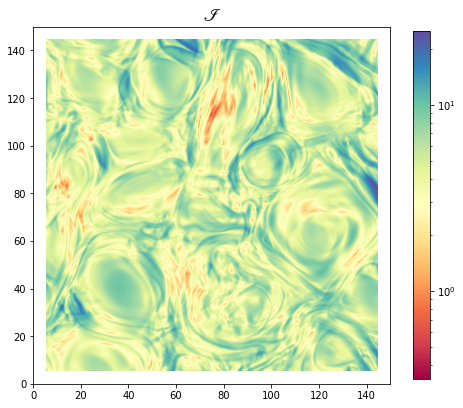
\includegraphics[width=0.45\textwidth]{pvi_2dpp.png}
				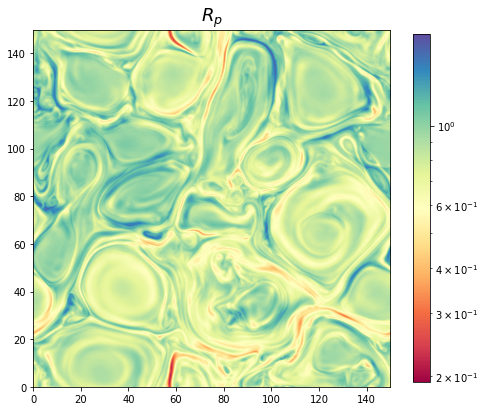
\includegraphics[width=0.45\textwidth]{rp_2dpp.png}
				\caption{PVI (on the left) and associated $R_p$ for 2D simulation (in plane magnetic field fluctuations).}
				\label{fig:pvi2dpp}
			\end{center}
		\end{figure*}

		\begin{figure*}
			\begin{center}
				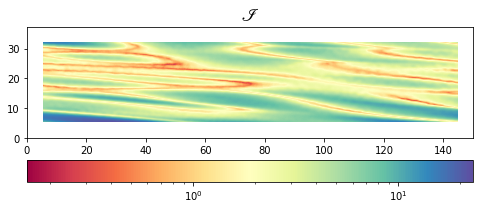
\includegraphics[width=0.45\textwidth]{pvi_2dip.png}
				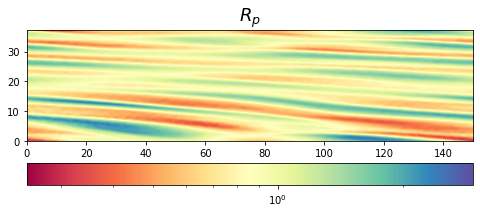
\includegraphics[width=0.45\textwidth]{rp_2dip.png}
				\caption{PVI (on the left) and associated $R_p$ for 2D simulation (out of plane magnetic field fluctuations).}
				\label{fig:fig:pvi2dip}
			\end{center}
		\end{figure*}

\clearpage
%\bibliographystyle{aasjournal}

%\begin{thebibliography}{}
\bibliography{Papers.bib}

%\end{thebibliography}


\end{document}
